\documentclass[1p]{elsarticle_modified}
%\bibliographystyle{elsarticle-num}

%\usepackage[colorlinks]{hyperref}
%\usepackage{abbrmath_seonhwa} %\Abb, \Ascr, \Acal ,\Abf, \Afrak
\usepackage{amsfonts}
\usepackage{amssymb}
\usepackage{amsmath}
\usepackage{amsthm}
\usepackage{scalefnt}
\usepackage{amsbsy}
\usepackage{kotex}
\usepackage{caption}
\usepackage{subfig}
\usepackage{color}
\usepackage{graphicx}
\usepackage{xcolor} %% white, black, red, green, blue, cyan, magenta, yellow
\usepackage{float}
\usepackage{setspace}
\usepackage{hyperref}

\usepackage{tikz}
\usetikzlibrary{arrows}

\usepackage{multirow}
\usepackage{array} % fixed length table
\usepackage{hhline}

%%%%%%%%%%%%%%%%%%%%%
\makeatletter
\renewcommand*\env@matrix[1][\arraystretch]{%
	\edef\arraystretch{#1}%
	\hskip -\arraycolsep
	\let\@ifnextchar\new@ifnextchar
	\array{*\c@MaxMatrixCols c}}
\makeatother %https://tex.stackexchange.com/questions/14071/how-can-i-increase-the-line-spacing-in-a-matrix
%%%%%%%%%%%%%%%

\usepackage[normalem]{ulem}

\newcommand{\msout}[1]{\ifmmode\text{\sout{\ensuremath{#1}}}\else\sout{#1}\fi}
%SOURCE: \msout is \stkout macro in https://tex.stackexchange.com/questions/20609/strikeout-in-math-mode

\newcommand{\cancel}[1]{
	\ifmmode
	{\color{red}\msout{#1}}
	\else
	{\color{red}\sout{#1}}
	\fi
}

\newcommand{\add}[1]{
	{\color{blue}\uwave{#1}}
}

\newcommand{\replace}[2]{
	\ifmmode
	{\color{red}\msout{#1}}{\color{blue}\uwave{#2}}
	\else
	{\color{red}\sout{#1}}{\color{blue}\uwave{#2}}
	\fi
}

\newcommand{\Sol}{\mathcal{S}} %segment
\newcommand{\D}{D} %diagram
\newcommand{\A}{\mathcal{A}} %arc


%%%%%%%%%%%%%%%%%%%%%%%%%%%%%5 test

\def\sl{\operatorname{\textup{SL}}(2,\Cbb)}
\def\psl{\operatorname{\textup{PSL}}(2,\Cbb)}
\def\quan{\mkern 1mu \triangleright \mkern 1mu}

\theoremstyle{definition}
\newtheorem{thm}{Theorem}[section]
\newtheorem{prop}[thm]{Proposition}
\newtheorem{lem}[thm]{Lemma}
\newtheorem{ques}[thm]{Question}
\newtheorem{cor}[thm]{Corollary}
\newtheorem{defn}[thm]{Definition}
\newtheorem{exam}[thm]{Example}
\newtheorem{rmk}[thm]{Remark}
\newtheorem{alg}[thm]{Algorithm}

\newcommand{\I}{\sqrt{-1}}
\begin{document}

%\begin{frontmatter}
%
%\title{Boundary parabolic representations of knots up to 8 crossings}
%
%%% Group authors per affiliation:
%\author{Yunhi Cho} 
%\address{Department of Mathematics, University of Seoul, Seoul, Korea}
%\ead{yhcho@uos.ac.kr}
%
%
%\author{Seonhwa Kim} %\fnref{s_kim}}
%\address{Center for Geometry and Physics, Institute for Basic Science, Pohang, 37673, Korea}
%\ead{ryeona17@ibs.re.kr}
%
%\author{Hyuk Kim}
%\address{Department of Mathematical Sciences, Seoul National University, Seoul 08826, Korea}
%\ead{hyukkim@snu.ac.kr}
%
%\author{Seokbeom Yoon}
%\address{Department of Mathematical Sciences, Seoul National University, Seoul, 08826,  Korea}
%\ead{sbyoon15@snu.ac.kr}
%
%\begin{abstract}
%We find all boundary parabolic representation of knots up to 8 crossings.
%
%\end{abstract}
%\begin{keyword}
%    \MSC[2010] 57M25 
%\end{keyword}
%
%\end{frontmatter}

%\linenumbers
%\tableofcontents
%
\newcommand\colored[1]{\textcolor{white}{\rule[-0.35ex]{0.8em}{1.4ex}}\kern-0.8em\color{red} #1}%
%\newcommand\colored[1]{\textcolor{white}{ #1}\kern-2.17ex	\textcolor{white}{ #1}\kern-1.81ex	\textcolor{white}{ #1}\kern-2.15ex\color{red}#1	}

{\Large $\underline{12n_{0674}~(K12n_{0674})}$}

\setlength{\tabcolsep}{10pt}
\renewcommand{\arraystretch}{1.6}
\vspace{1cm}\begin{tabular}{m{100pt}>{\centering\arraybackslash}m{274pt}}
\multirow{5}{120pt}{
	\centering
	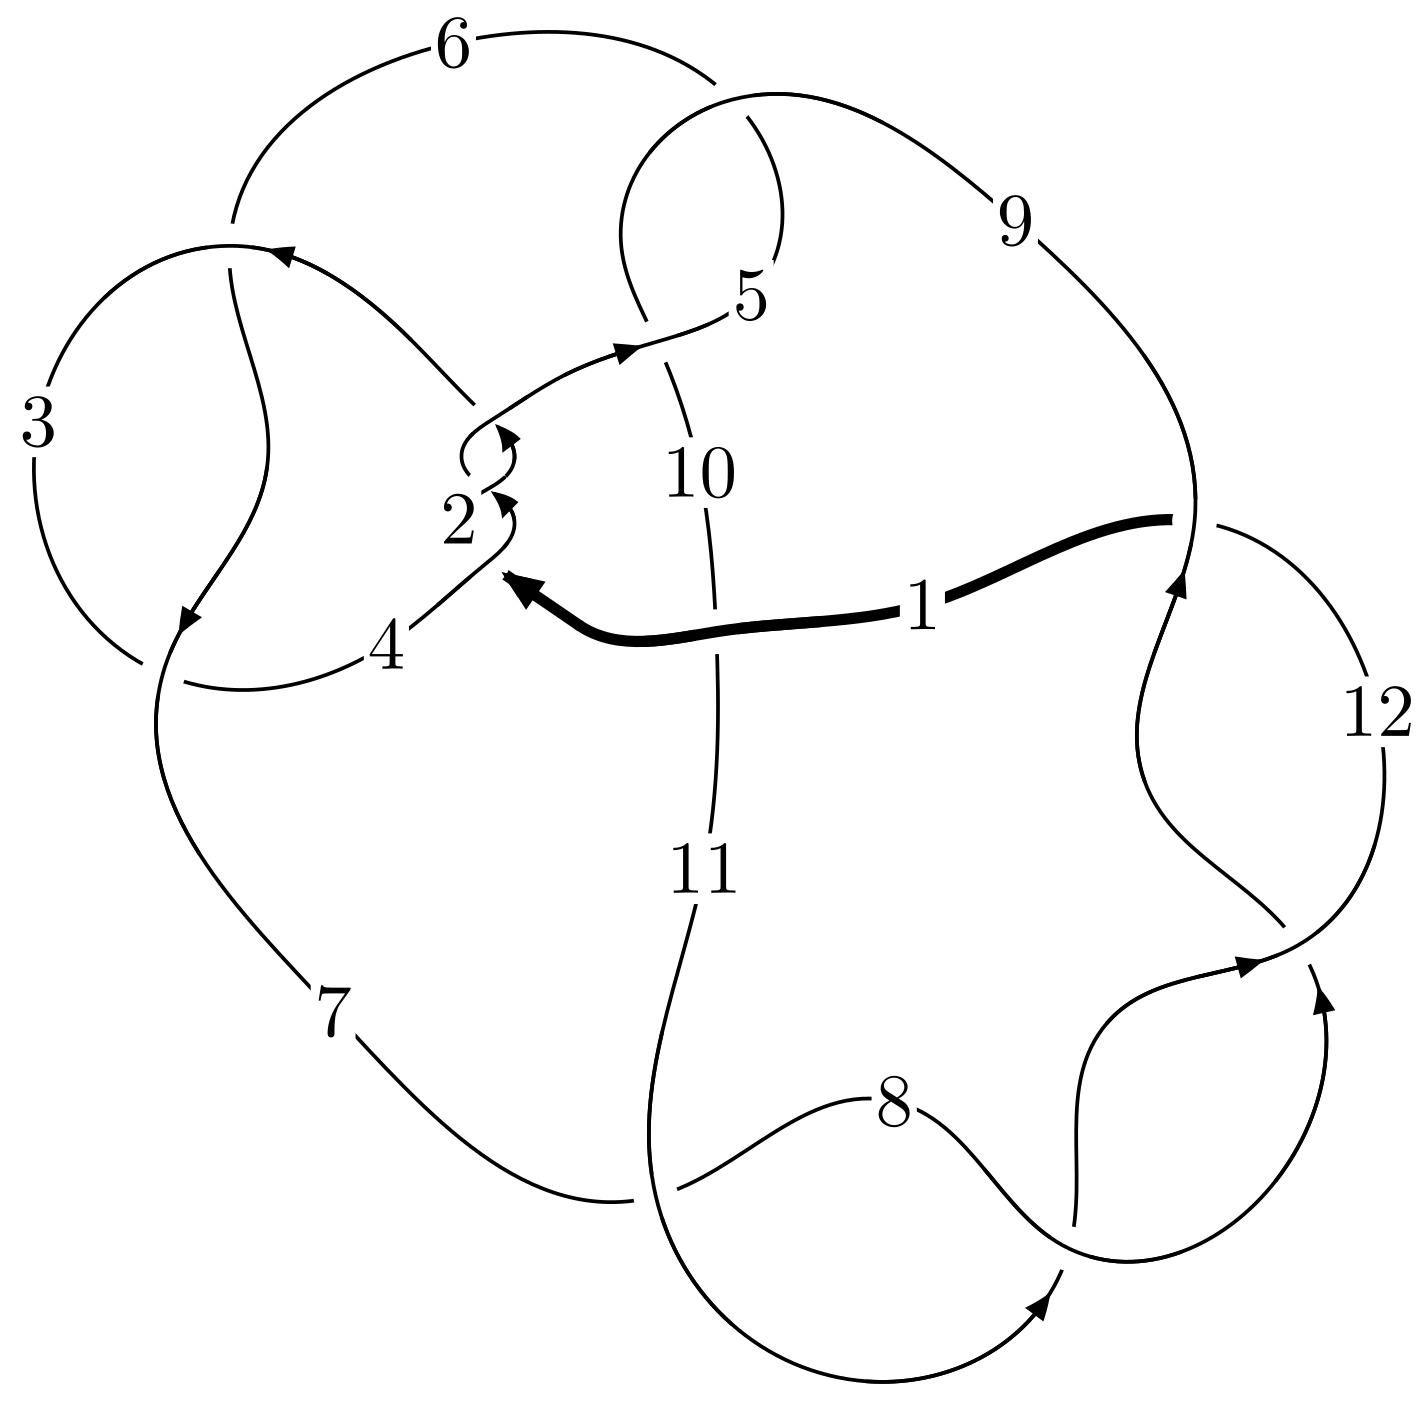
\includegraphics[width=112pt]{../../../GIT/diagram.site/Diagrams/png/2763_12n_0674.png}\\
\ \ \ A knot diagram\footnotemark}&
\allowdisplaybreaks
\textbf{Linearized knot diagam} \\
\cline{2-2}
 &
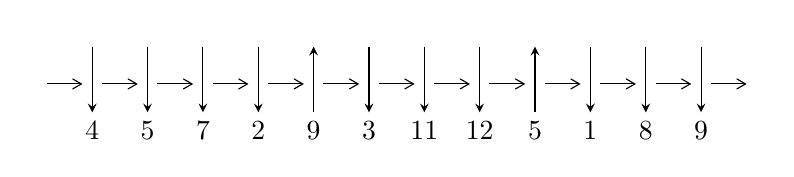
\begin{tikzpicture}[x=20pt, y=17pt]
	% nodes
	\node (C0) at (0, 0) {};
	\node (C1) at (1, 0) {};
	\node (C1U) at (1, +1) {};
	\node (C1D) at (1, -1) {4};

	\node (C2) at (2, 0) {};
	\node (C2U) at (2, +1) {};
	\node (C2D) at (2, -1) {5};

	\node (C3) at (3, 0) {};
	\node (C3U) at (3, +1) {};
	\node (C3D) at (3, -1) {7};

	\node (C4) at (4, 0) {};
	\node (C4U) at (4, +1) {};
	\node (C4D) at (4, -1) {2};

	\node (C5) at (5, 0) {};
	\node (C5U) at (5, +1) {};
	\node (C5D) at (5, -1) {9};

	\node (C6) at (6, 0) {};
	\node (C6U) at (6, +1) {};
	\node (C6D) at (6, -1) {3};

	\node (C7) at (7, 0) {};
	\node (C7U) at (7, +1) {};
	\node (C7D) at (7, -1) {11};

	\node (C8) at (8, 0) {};
	\node (C8U) at (8, +1) {};
	\node (C8D) at (8, -1) {12};

	\node (C9) at (9, 0) {};
	\node (C9U) at (9, +1) {};
	\node (C9D) at (9, -1) {5};

	\node (C10) at (10, 0) {};
	\node (C10U) at (10, +1) {};
	\node (C10D) at (10, -1) {1};

	\node (C11) at (11, 0) {};
	\node (C11U) at (11, +1) {};
	\node (C11D) at (11, -1) {8};

	\node (C12) at (12, 0) {};
	\node (C12U) at (12, +1) {};
	\node (C12D) at (12, -1) {9};
	\node (C13) at (13, 0) {};

	% arrows
	\draw[->,>={angle 60}]
	(C0) edge (C1) (C1) edge (C2) (C2) edge (C3) (C3) edge (C4) (C4) edge (C5) (C5) edge (C6) (C6) edge (C7) (C7) edge (C8) (C8) edge (C9) (C9) edge (C10) (C10) edge (C11) (C11) edge (C12) (C12) edge (C13) ;	\draw[->,>=stealth]
	(C1U) edge (C1D) (C2U) edge (C2D) (C3U) edge (C3D) (C4U) edge (C4D) (C5D) edge (C5U) (C6U) edge (C6D) (C7U) edge (C7D) (C8U) edge (C8D) (C9D) edge (C9U) (C10U) edge (C10D) (C11U) edge (C11D) (C12U) edge (C12D) ;
	\end{tikzpicture} \\
\hhline{~~} \\& 
\textbf{Solving Sequence} \\ \cline{2-2} 
 &
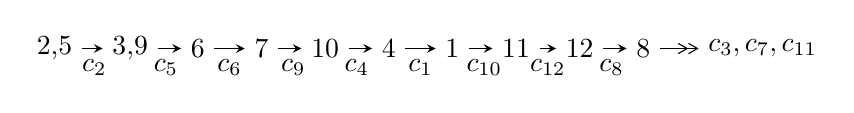
\begin{tikzpicture}[x=23pt, y=7pt]
	% node
	\node (A0) at (-1/8, 0) {2,5};
	\node (A1) at (17/16, 0) {3,9};
	\node (A2) at (17/8, 0) {6};
	\node (A3) at (25/8, 0) {7};
	\node (A4) at (33/8, 0) {10};
	\node (A5) at (41/8, 0) {4};
	\node (A6) at (49/8, 0) {1};
	\node (A7) at (57/8, 0) {11};
	\node (A8) at (65/8, 0) {12};
	\node (A9) at (73/8, 0) {8};
	\node (C1) at (1/2, -1) {$c_{2}$};
	\node (C2) at (13/8, -1) {$c_{5}$};
	\node (C3) at (21/8, -1) {$c_{6}$};
	\node (C4) at (29/8, -1) {$c_{9}$};
	\node (C5) at (37/8, -1) {$c_{4}$};
	\node (C6) at (45/8, -1) {$c_{1}$};
	\node (C7) at (53/8, -1) {$c_{10}$};
	\node (C8) at (61/8, -1) {$c_{12}$};
	\node (C9) at (69/8, -1) {$c_{8}$};
	\node (A10) at (11, 0) {$c_{3},c_{7},c_{11}$};

	% edge
	\draw[->,>=stealth]	
	(A0) edge (A1) (A1) edge (A2) (A2) edge (A3) (A3) edge (A4) (A4) edge (A5) (A5) edge (A6) (A6) edge (A7) (A7) edge (A8) (A8) edge (A9) ;
	\draw[->>,>={angle 60}]	
	(A9) edge (A10);
\end{tikzpicture} \\ 

\end{tabular} \\

\footnotetext{
The image of knot diagram is generated by the software ``\textbf{Draw programme}" developed by Andrew Bartholomew(\url{http://www.layer8.co.uk/maths/draw/index.htm\#Running-draw}), where we modified some parts for our purpose(\url{https://github.com/CATsTAILs/LinksPainter}).
}\phantom \\ \newline 
\centering \textbf{Ideals for irreducible components\footnotemark of $X_{\text{par}}$} 
 
\begin{align*}
I^u_{1}&=\langle 
-8.95545\times10^{24} u^{41}-2.72305\times10^{25} u^{40}+\cdots+2.32080\times10^{24} b+1.04846\times10^{24},\\
\phantom{I^u_{1}}&\phantom{= \langle  }-2.76332\times10^{24} u^{41}-4.41119\times10^{24} u^{40}+\cdots+2.32080\times10^{24} a+2.12642\times10^{25},\\
\phantom{I^u_{1}}&\phantom{= \langle  }u^{42}+4 u^{41}+\cdots+14 u-1\rangle \\
I^u_{2}&=\langle 
b+1,\;a,\;u^2+u-1\rangle \\
I^u_{3}&=\langle 
b- u-2,\;a,\;u^2+u-1\rangle \\
I^u_{4}&=\langle 
b,\;a+1,\;u-1\rangle \\
\\
\end{align*}
\raggedright * 4 irreducible components of $\dim_{\mathbb{C}}=0$, with total 47 representations.\\
\footnotetext{All coefficients of polynomials are rational numbers. But the coefficients are sometimes approximated in decimal forms when there is not enough margin.}
\newpage
\renewcommand{\arraystretch}{1}
\centering \section*{I. $I^u_{1}= \langle -8.96\times10^{24} u^{41}-2.72\times10^{25} u^{40}+\cdots+2.32\times10^{24} b+1.05\times10^{24},\;-2.76\times10^{24} u^{41}-4.41\times10^{24} u^{40}+\cdots+2.32\times10^{24} a+2.13\times10^{25},\;u^{42}+4 u^{41}+\cdots+14 u-1 \rangle$}
\flushleft \textbf{(i) Arc colorings}\\
\begin{tabular}{m{7pt} m{180pt} m{7pt} m{180pt} }
\flushright $a_{2}=$&$\begin{pmatrix}1\\0\end{pmatrix}$ \\
\flushright $a_{5}=$&$\begin{pmatrix}0\\u\end{pmatrix}$ \\
\flushright $a_{3}=$&$\begin{pmatrix}1\\u^2\end{pmatrix}$ \\
\flushright $a_{9}=$&$\begin{pmatrix}1.19067 u^{41}+1.90072 u^{40}+\cdots+60.6010 u-9.16243\\3.85878 u^{41}+11.7332 u^{40}+\cdots+22.3744 u-0.451767\end{pmatrix}$ \\
\flushright $a_{6}=$&$\begin{pmatrix}-0.105132 u^{41}-0.0128494 u^{40}+\cdots-34.8388 u+4.84834\\-0.848783 u^{41}-2.84893 u^{40}+\cdots-15.2500 u+0.685419\end{pmatrix}$ \\
\flushright $a_{7}=$&$\begin{pmatrix}0.978378 u^{41}+2.65739 u^{40}+\cdots-25.4014 u+4.57060\\1.25612 u^{41}+2.68484 u^{40}+\cdots+9.12669 u-0.978378\end{pmatrix}$ \\
\flushright $a_{10}=$&$\begin{pmatrix}1.19067 u^{41}+1.90072 u^{40}+\cdots+60.6010 u-9.16243\\0.716340 u^{41}+3.10175 u^{40}+\cdots-18.8840 u+2.41021\end{pmatrix}$ \\
\flushright $a_{4}=$&$\begin{pmatrix}u\\u\end{pmatrix}$ \\
\flushright $a_{1}=$&$\begin{pmatrix}- u^2+1\\- u^2\end{pmatrix}$ \\
\flushright $a_{11}=$&$\begin{pmatrix}2.55115 u^{41}+4.97020 u^{40}+\cdots+92.6692 u-12.2894\\5.70141 u^{41}+16.8545 u^{40}+\cdots+38.1516 u-1.40486\end{pmatrix}$ \\
\flushright $a_{12}=$&$\begin{pmatrix}-0.546898 u^{41}-1.27331 u^{40}+\cdots-34.6001 u+6.91046\\-1.81884 u^{41}-4.93743 u^{40}+\cdots-37.5544 u+2.14072\end{pmatrix}$ \\
\flushright $a_{8}=$&$\begin{pmatrix}-0.0791429 u^{41}+0.265882 u^{40}+\cdots-13.4298 u-0.240862\\-0.00645021 u^{41}-0.654296 u^{40}+\cdots+17.6519 u-1.13841\end{pmatrix}$\\&\end{tabular}
\flushleft \textbf{(ii) Obstruction class $= -1$}\\~\\
\flushleft \textbf{(iii) Cusp Shapes $= \frac{8061029839060072009079083}{2320801929915461688487812} u^{41}+\frac{4209450828705721840877893}{580200482478865422121953} u^{40}+\cdots+\frac{55742079073151734903802548}{580200482478865422121953} u-\frac{31967218726697708827064461}{2320801929915461688487812}$}\\~\\
\newpage\renewcommand{\arraystretch}{1}
\flushleft \textbf{(iv) u-Polynomials at the component}\newline \\
\begin{tabular}{m{50pt}|m{274pt}}
Crossings & \hspace{64pt}u-Polynomials at each crossing \\
\hline $$\begin{aligned}c_{1},c_{2},c_{4}\end{aligned}$$&$\begin{aligned}
&u^{42}-4 u^{41}+\cdots-14 u-1
\end{aligned}$\\
\hline $$\begin{aligned}c_{3},c_{6}\end{aligned}$$&$\begin{aligned}
&u^{42}+3 u^{41}+\cdots-15 u^2+2
\end{aligned}$\\
\hline $$\begin{aligned}c_{5},c_{9}\end{aligned}$$&$\begin{aligned}
&u^{42}-2 u^{41}+\cdots-32 u-16
\end{aligned}$\\
\hline $$\begin{aligned}c_{7},c_{8},c_{11}\\c_{12}\end{aligned}$$&$\begin{aligned}
&u^{42}+4 u^{41}+\cdots-10 u+1
\end{aligned}$\\
\hline $$\begin{aligned}c_{10}\end{aligned}$$&$\begin{aligned}
&u^{42}-8 u^{41}+\cdots-11932 u-167
\end{aligned}$\\
\hline
\end{tabular}\\~\\
\newpage\renewcommand{\arraystretch}{1}
\flushleft \textbf{(v) Riley Polynomials at the component}\newline \\
\begin{tabular}{m{50pt}|m{274pt}}
Crossings & \hspace{64pt}Riley Polynomials at each crossing \\
\hline $$\begin{aligned}c_{1},c_{2},c_{4}\end{aligned}$$&$\begin{aligned}
&y^{42}-36 y^{41}+\cdots-78 y+1
\end{aligned}$\\
\hline $$\begin{aligned}c_{3},c_{6}\end{aligned}$$&$\begin{aligned}
&y^{42}-15 y^{41}+\cdots-60 y+4
\end{aligned}$\\
\hline $$\begin{aligned}c_{5},c_{9}\end{aligned}$$&$\begin{aligned}
&y^{42}-26 y^{41}+\cdots-7296 y+256
\end{aligned}$\\
\hline $$\begin{aligned}c_{7},c_{8},c_{11}\\c_{12}\end{aligned}$$&$\begin{aligned}
&y^{42}-48 y^{41}+\cdots-154 y+1
\end{aligned}$\\
\hline $$\begin{aligned}c_{10}\end{aligned}$$&$\begin{aligned}
&y^{42}+12 y^{41}+\cdots-132872662 y+27889
\end{aligned}$\\
\hline
\end{tabular}\\~\\
\newpage\flushleft \textbf{(vi) Complex Volumes and Cusp Shapes}
$$\begin{array}{c|c|c}  
\text{Solutions to }I^u_{1}& \I (\text{vol} + \sqrt{-1}CS) & \text{Cusp shape}\\
 \hline 
\begin{aligned}
u &= \phantom{-}0.238287 + 0.993330 I \\
a &= -0.256688 - 1.363750 I \\
b &= \phantom{-}0.448503 - 0.389957 I\end{aligned}
 & -3.87928 - 8.09823 I & -11.51544 + 5.48666 I \\ \hline\begin{aligned}
u &= \phantom{-}0.238287 - 0.993330 I \\
a &= -0.256688 + 1.363750 I \\
b &= \phantom{-}0.448503 + 0.389957 I\end{aligned}
 & -3.87928 + 8.09823 I & -11.51544 - 5.48666 I \\ \hline\begin{aligned}
u &= \phantom{-}1.060390 + 0.045339 I \\
a &= \phantom{-}0.258751 + 0.376269 I \\
b &= -0.47464 + 2.91568 I\end{aligned}
 & -2.71639 - 0.33816 I & -4.0081 - 13.7250 I \\ \hline\begin{aligned}
u &= \phantom{-}1.060390 - 0.045339 I \\
a &= \phantom{-}0.258751 - 0.376269 I \\
b &= -0.47464 - 2.91568 I\end{aligned}
 & -2.71639 + 0.33816 I & -4.0081 + 13.7250 I \\ \hline\begin{aligned}
u &= \phantom{-}0.106704 + 0.918803 I \\
a &= \phantom{-}0.26496 + 1.45259 I \\
b &= -0.086830 + 0.297294 I\end{aligned}
 & \phantom{-}3.36143 - 5.24537 I & -7.74689 + 6.20199 I \\ \hline\begin{aligned}
u &= \phantom{-}0.106704 - 0.918803 I \\
a &= \phantom{-}0.26496 - 1.45259 I \\
b &= -0.086830 - 0.297294 I\end{aligned}
 & \phantom{-}3.36143 + 5.24537 I & -7.74689 - 6.20199 I \\ \hline\begin{aligned}
u &= \phantom{-}1.147150 + 0.210471 I \\
a &= -0.302824 - 0.583834 I \\
b &= -0.04054 - 3.07018 I\end{aligned}
 & -10.17350 - 0.96398 I & -18.1472 - 3.3317 I \\ \hline\begin{aligned}
u &= \phantom{-}1.147150 - 0.210471 I \\
a &= -0.302824 + 0.583834 I \\
b &= -0.04054 + 3.07018 I\end{aligned}
 & -10.17350 + 0.96398 I & -18.1472 + 3.3317 I \\ \hline\begin{aligned}
u &= -0.049648 + 0.825086 I \\
a &= -0.32016 - 1.57337 I \\
b &= -0.281826 - 0.254570 I\end{aligned}
 & \phantom{-}4.07908 - 1.05002 I & -5.39403 - 0.20283 I \\ \hline\begin{aligned}
u &= -0.049648 - 0.825086 I \\
a &= -0.32016 + 1.57337 I \\
b &= -0.281826 + 0.254570 I\end{aligned}
 & \phantom{-}4.07908 + 1.05002 I & -5.39403 + 0.20283 I\\
 \hline 
 \end{array}$$\newpage$$\begin{array}{c|c|c}  
\text{Solutions to }I^u_{1}& \I (\text{vol} + \sqrt{-1}CS) & \text{Cusp shape}\\
 \hline 
\begin{aligned}
u &= -1.168990 + 0.199735 I \\
a &= \phantom{-}1.249760 + 0.642269 I \\
b &= \phantom{-}1.006910 + 0.970924 I\end{aligned}
 & -3.90037 + 1.20976 I & -15.7241 - 4.9251 I \\ \hline\begin{aligned}
u &= -1.168990 - 0.199735 I \\
a &= \phantom{-}1.249760 - 0.642269 I \\
b &= \phantom{-}1.006910 - 0.970924 I\end{aligned}
 & -3.90037 - 1.20976 I & -15.7241 + 4.9251 I \\ \hline\begin{aligned}
u &= -0.314243 + 0.696899 I \\
a &= \phantom{-}0.56188 + 1.69109 I \\
b &= \phantom{-}0.733268 + 0.302512 I\end{aligned}
 & -1.53621 + 1.78916 I & -8.56962 - 1.59900 I \\ \hline\begin{aligned}
u &= -0.314243 - 0.696899 I \\
a &= \phantom{-}0.56188 - 1.69109 I \\
b &= \phantom{-}0.733268 - 0.302512 I\end{aligned}
 & -1.53621 - 1.78916 I & -8.56962 + 1.59900 I \\ \hline\begin{aligned}
u &= -1.244640 + 0.090513 I \\
a &= \phantom{-}0.277107 - 1.196450 I \\
b &= \phantom{-}0.18513 - 2.18299 I\end{aligned}
 & -4.74961 + 2.33690 I & -17.2595 - 5.0904 I \\ \hline\begin{aligned}
u &= -1.244640 - 0.090513 I \\
a &= \phantom{-}0.277107 + 1.196450 I \\
b &= \phantom{-}0.18513 + 2.18299 I\end{aligned}
 & -4.74961 - 2.33690 I & -17.2595 + 5.0904 I \\ \hline\begin{aligned}
u &= \phantom{-}1.157940 + 0.481959 I \\
a &= -0.776705 + 0.303294 I \\
b &= -0.979087 + 0.599725 I\end{aligned}
 & \phantom{-}0.121226 + 0.269727 I & -8.00000 - 3.11579 I \\ \hline\begin{aligned}
u &= \phantom{-}1.157940 - 0.481959 I \\
a &= -0.776705 - 0.303294 I \\
b &= -0.979087 - 0.599725 I\end{aligned}
 & \phantom{-}0.121226 - 0.269727 I & -8.00000 + 3.11579 I \\ \hline\begin{aligned}
u &= \phantom{-}1.057900 + 0.692054 I \\
a &= \phantom{-}0.907159 - 0.280920 I \\
b &= \phantom{-}0.898757 + 0.137083 I\end{aligned}
 & -6.34245 + 2.32209 I & -13.28779 + 0. I\phantom{ +0.000000I} \\ \hline\begin{aligned}
u &= \phantom{-}1.057900 - 0.692054 I \\
a &= \phantom{-}0.907159 + 0.280920 I \\
b &= \phantom{-}0.898757 - 0.137083 I\end{aligned}
 & -6.34245 - 2.32209 I & -13.28779 + 0. I\phantom{ +0.000000I}\\
 \hline 
 \end{array}$$\newpage$$\begin{array}{c|c|c}  
\text{Solutions to }I^u_{1}& \I (\text{vol} + \sqrt{-1}CS) & \text{Cusp shape}\\
 \hline 
\begin{aligned}
u &= \phantom{-}0.722474\phantom{ +0.000000I} \\
a &= -0.399724\phantom{ +0.000000I} \\
b &= \phantom{-}0.258120\phantom{ +0.000000I}\end{aligned}
 & -1.09552\phantom{ +0.000000I} & -8.48520\phantom{ +0.000000I} \\ \hline\begin{aligned}
u &= -1.245000 + 0.375694 I \\
a &= -0.928202 - 0.816670 I \\
b &= -1.17456 - 1.47199 I\end{aligned}
 & \phantom{-}0.37946 + 5.36737 I & \phantom{-0.000000 } 0 \\ \hline\begin{aligned}
u &= -1.245000 - 0.375694 I \\
a &= -0.928202 + 0.816670 I \\
b &= -1.17456 + 1.47199 I\end{aligned}
 & \phantom{-}0.37946 - 5.36737 I & \phantom{-0.000000 } 0 \\ \hline\begin{aligned}
u &= -1.31935\phantom{ +0.000000I} \\
a &= -1.01441\phantom{ +0.000000I} \\
b &= -0.0413566\phantom{ +0.000000I}\end{aligned}
 & -14.8036\phantom{ +0.000000I} & -18.1030\phantom{ +0.000000I} \\ \hline\begin{aligned}
u &= -1.308760 + 0.256721 I \\
a &= -0.597154 + 0.929246 I \\
b &= -0.45147 + 2.20887 I\end{aligned}
 & -11.72140 + 5.51488 I & \phantom{-0.000000 } 0 \\ \hline\begin{aligned}
u &= -1.308760 - 0.256721 I \\
a &= -0.597154 - 0.929246 I \\
b &= -0.45147 - 2.20887 I\end{aligned}
 & -11.72140 - 5.51488 I & \phantom{-0.000000 } 0 \\ \hline\begin{aligned}
u &= \phantom{-}0.126480 + 0.653902 I \\
a &= \phantom{-}1.60072 - 0.06394 I \\
b &= -0.579441 - 0.327004 I\end{aligned}
 & -7.23822 - 2.23215 I & -12.66894 + 2.87063 I \\ \hline\begin{aligned}
u &= \phantom{-}0.126480 - 0.653902 I \\
a &= \phantom{-}1.60072 + 0.06394 I \\
b &= -0.579441 + 0.327004 I\end{aligned}
 & -7.23822 + 2.23215 I & -12.66894 - 2.87063 I \\ \hline\begin{aligned}
u &= \phantom{-}1.329240 + 0.371704 I \\
a &= \phantom{-}0.714985 - 0.404132 I \\
b &= \phantom{-}1.36849 - 1.26529 I\end{aligned}
 & -0.24891 - 3.25176 I & \phantom{-0.000000 } 0 \\ \hline\begin{aligned}
u &= \phantom{-}1.329240 - 0.371704 I \\
a &= \phantom{-}0.714985 + 0.404132 I \\
b &= \phantom{-}1.36849 + 1.26529 I\end{aligned}
 & -0.24891 + 3.25176 I & \phantom{-0.000000 } 0\\
 \hline 
 \end{array}$$\newpage$$\begin{array}{c|c|c}  
\text{Solutions to }I^u_{1}& \I (\text{vol} + \sqrt{-1}CS) & \text{Cusp shape}\\
 \hline 
\begin{aligned}
u &= -1.35150 + 0.42227 I \\
a &= \phantom{-}0.777238 + 0.800492 I \\
b &= \phantom{-}1.23840 + 1.87181 I\end{aligned}
 & -1.20516 + 10.04620 I & \phantom{-0.000000 } 0 \\ \hline\begin{aligned}
u &= -1.35150 - 0.42227 I \\
a &= \phantom{-}0.777238 - 0.800492 I \\
b &= \phantom{-}1.23840 - 1.87181 I\end{aligned}
 & -1.20516 - 10.04620 I & \phantom{-0.000000 } 0 \\ \hline\begin{aligned}
u &= \phantom{-}1.46265 + 0.31490 I \\
a &= -0.703570 + 0.478725 I \\
b &= -1.75849 + 1.73373 I\end{aligned}
 & -7.27437 - 5.59691 I & \phantom{-0.000000 } 0 \\ \hline\begin{aligned}
u &= \phantom{-}1.46265 - 0.31490 I \\
a &= -0.703570 - 0.478725 I \\
b &= -1.75849 - 1.73373 I\end{aligned}
 & -7.27437 + 5.59691 I & \phantom{-0.000000 } 0 \\ \hline\begin{aligned}
u &= -1.43580 + 0.43130 I \\
a &= -0.682703 - 0.780467 I \\
b &= -1.24611 - 2.24244 I\end{aligned}
 & -9.1607 + 13.1986 I & \phantom{-0.000000 } 0 \\ \hline\begin{aligned}
u &= -1.43580 - 0.43130 I \\
a &= -0.682703 + 0.780467 I \\
b &= -1.24611 + 2.24244 I\end{aligned}
 & -9.1607 - 13.1986 I & \phantom{-0.000000 } 0 \\ \hline\begin{aligned}
u &= \phantom{-}0.403841\phantom{ +0.000000I} \\
a &= \phantom{-}1.04866\phantom{ +0.000000I} \\
b &= -2.15536\phantom{ +0.000000I}\end{aligned}
 & -9.66299\phantom{ +0.000000I} & \phantom{-}4.31750\phantom{ +0.000000I} \\ \hline\begin{aligned}
u &= -1.64023\phantom{ +0.000000I} \\
a &= \phantom{-}0.220147\phantom{ +0.000000I} \\
b &= \phantom{-}0.661174\phantom{ +0.000000I}\end{aligned}
 & -9.70143\phantom{ +0.000000I} & \phantom{-0.000000 } 0 \\ \hline\begin{aligned}
u &= \phantom{-}0.152045 + 0.289588 I \\
a &= -1.95648 - 0.86091 I \\
b &= \phantom{-}0.166595 + 0.401559 I\end{aligned}
 & -0.703904 - 0.992275 I & -8.59202 + 6.89400 I \\ \hline\begin{aligned}
u &= \phantom{-}0.152045 - 0.289588 I \\
a &= -1.95648 + 0.86091 I \\
b &= \phantom{-}0.166595 - 0.401559 I\end{aligned}
 & -0.703904 + 0.992275 I & -8.59202 - 6.89400 I\\
 \hline 
 \end{array}$$\newpage$$\begin{array}{c|c|c}  
\text{Solutions to }I^u_{1}& \I (\text{vol} + \sqrt{-1}CS) & \text{Cusp shape}\\
 \hline 
\begin{aligned}
u &= -1.71883\phantom{ +0.000000I} \\
a &= -0.450881\phantom{ +0.000000I} \\
b &= -1.47918\phantom{ +0.000000I}\end{aligned}
 & -16.8863\phantom{ +0.000000I} & \phantom{-0.000000 } 0 \\ \hline\begin{aligned}
u &= \phantom{-}0.111686\phantom{ +0.000000I} \\
a &= -4.57994\phantom{ +0.000000I} \\
b &= \phantom{-}0.810470\phantom{ +0.000000I}\end{aligned}
 & -1.32929\phantom{ +0.000000I} & -5.96870\phantom{ +0.000000I}\\
 \hline 
 \end{array}$$\newpage\newpage\renewcommand{\arraystretch}{1}
\centering \section*{II. $I^u_{2}= \langle b+1,\;a,\;u^2+u-1 \rangle$}
\flushleft \textbf{(i) Arc colorings}\\
\begin{tabular}{m{7pt} m{180pt} m{7pt} m{180pt} }
\flushright $a_{2}=$&$\begin{pmatrix}1\\0\end{pmatrix}$ \\
\flushright $a_{5}=$&$\begin{pmatrix}0\\u\end{pmatrix}$ \\
\flushright $a_{3}=$&$\begin{pmatrix}1\\- u+1\end{pmatrix}$ \\
\flushright $a_{9}=$&$\begin{pmatrix}0\\-1\end{pmatrix}$ \\
\flushright $a_{6}=$&$\begin{pmatrix}0\\u\end{pmatrix}$ \\
\flushright $a_{7}=$&$\begin{pmatrix}- u\\- u+1\end{pmatrix}$ \\
\flushright $a_{10}=$&$\begin{pmatrix}0\\-1\end{pmatrix}$ \\
\flushright $a_{4}=$&$\begin{pmatrix}u\\u\end{pmatrix}$ \\
\flushright $a_{1}=$&$\begin{pmatrix}u\\u-1\end{pmatrix}$ \\
\flushright $a_{11}=$&$\begin{pmatrix}- u+1\\-2 u\end{pmatrix}$ \\
\flushright $a_{12}=$&$\begin{pmatrix}u\\-1\end{pmatrix}$ \\
\flushright $a_{8}=$&$\begin{pmatrix}u-1\\u-1\end{pmatrix}$\\&\end{tabular}
\flushleft \textbf{(ii) Obstruction class $= 1$}\\~\\
\flushleft \textbf{(iii) Cusp Shapes $= -21$}\\~\\
\newpage\renewcommand{\arraystretch}{1}
\flushleft \textbf{(iv) u-Polynomials at the component}\newline \\
\begin{tabular}{m{50pt}|m{274pt}}
Crossings & \hspace{64pt}u-Polynomials at each crossing \\
\hline $$\begin{aligned}c_{1},c_{2},c_{3}\\c_{7},c_{8},c_{10}\end{aligned}$$&$\begin{aligned}
&u^2+u-1
\end{aligned}$\\
\hline $$\begin{aligned}c_{4},c_{6},c_{11}\\c_{12}\end{aligned}$$&$\begin{aligned}
&u^2- u-1
\end{aligned}$\\
\hline $$\begin{aligned}c_{5},c_{9}\end{aligned}$$&$\begin{aligned}
&u^2
\end{aligned}$\\
\hline
\end{tabular}\\~\\
\newpage\renewcommand{\arraystretch}{1}
\flushleft \textbf{(v) Riley Polynomials at the component}\newline \\
\begin{tabular}{m{50pt}|m{274pt}}
Crossings & \hspace{64pt}Riley Polynomials at each crossing \\
\hline $$\begin{aligned}c_{1},c_{2},c_{3}\\c_{4},c_{6},c_{7}\\c_{8},c_{10},c_{11}\\c_{12}\end{aligned}$$&$\begin{aligned}
&y^2-3 y+1
\end{aligned}$\\
\hline $$\begin{aligned}c_{5},c_{9}\end{aligned}$$&$\begin{aligned}
&y^2
\end{aligned}$\\
\hline
\end{tabular}\\~\\
\newpage\flushleft \textbf{(vi) Complex Volumes and Cusp Shapes}
$$\begin{array}{c|c|c}  
\text{Solutions to }I^u_{2}& \I (\text{vol} + \sqrt{-1}CS) & \text{Cusp shape}\\
 \hline 
\begin{aligned}
u &= \phantom{-}0.618034\phantom{ +0.000000I} \\
a &= \phantom{-0.000000 } 0 \\
b &= -1.00000\phantom{ +0.000000I}\end{aligned}
 & -1.97392\phantom{ +0.000000I} & -21.0000\phantom{ +0.000000I} \\ \hline\begin{aligned}
u &= -1.61803\phantom{ +0.000000I} \\
a &= \phantom{-0.000000 } 0 \\
b &= -1.00000\phantom{ +0.000000I}\end{aligned}
 & -17.7653\phantom{ +0.000000I} & -21.0000\phantom{ +0.000000I}\\
 \hline 
 \end{array}$$\newpage\newpage\renewcommand{\arraystretch}{1}
\centering \section*{III. $I^u_{3}= \langle b- u-2,\;a,\;u^2+u-1 \rangle$}
\flushleft \textbf{(i) Arc colorings}\\
\begin{tabular}{m{7pt} m{180pt} m{7pt} m{180pt} }
\flushright $a_{2}=$&$\begin{pmatrix}1\\0\end{pmatrix}$ \\
\flushright $a_{5}=$&$\begin{pmatrix}0\\u\end{pmatrix}$ \\
\flushright $a_{3}=$&$\begin{pmatrix}1\\- u+1\end{pmatrix}$ \\
\flushright $a_{9}=$&$\begin{pmatrix}0\\u+2\end{pmatrix}$ \\
\flushright $a_{6}=$&$\begin{pmatrix}0\\u\end{pmatrix}$ \\
\flushright $a_{7}=$&$\begin{pmatrix}- u\\- u+1\end{pmatrix}$ \\
\flushright $a_{10}=$&$\begin{pmatrix}0\\u+2\end{pmatrix}$ \\
\flushright $a_{4}=$&$\begin{pmatrix}u\\u\end{pmatrix}$ \\
\flushright $a_{1}=$&$\begin{pmatrix}u\\u-1\end{pmatrix}$ \\
\flushright $a_{11}=$&$\begin{pmatrix}-1\\2 u+2\end{pmatrix}$ \\
\flushright $a_{12}=$&$\begin{pmatrix}u\\- u-4\end{pmatrix}$ \\
\flushright $a_{8}=$&$\begin{pmatrix}1\\-3 u-3\end{pmatrix}$\\&\end{tabular}
\flushleft \textbf{(ii) Obstruction class $= 1$}\\~\\
\flushleft \textbf{(iii) Cusp Shapes $= -36$}\\~\\
\newpage\renewcommand{\arraystretch}{1}
\flushleft \textbf{(iv) u-Polynomials at the component}\newline \\
\begin{tabular}{m{50pt}|m{274pt}}
Crossings & \hspace{64pt}u-Polynomials at each crossing \\
\hline $$\begin{aligned}c_{1},c_{2},c_{3}\\c_{7},c_{8},c_{10}\end{aligned}$$&$\begin{aligned}
&u^2+u-1
\end{aligned}$\\
\hline $$\begin{aligned}c_{4},c_{6},c_{11}\\c_{12}\end{aligned}$$&$\begin{aligned}
&u^2- u-1
\end{aligned}$\\
\hline $$\begin{aligned}c_{5},c_{9}\end{aligned}$$&$\begin{aligned}
&u^2
\end{aligned}$\\
\hline
\end{tabular}\\~\\
\newpage\renewcommand{\arraystretch}{1}
\flushleft \textbf{(v) Riley Polynomials at the component}\newline \\
\begin{tabular}{m{50pt}|m{274pt}}
Crossings & \hspace{64pt}Riley Polynomials at each crossing \\
\hline $$\begin{aligned}c_{1},c_{2},c_{3}\\c_{4},c_{6},c_{7}\\c_{8},c_{10},c_{11}\\c_{12}\end{aligned}$$&$\begin{aligned}
&y^2-3 y+1
\end{aligned}$\\
\hline $$\begin{aligned}c_{5},c_{9}\end{aligned}$$&$\begin{aligned}
&y^2
\end{aligned}$\\
\hline
\end{tabular}\\~\\
\newpage\flushleft \textbf{(vi) Complex Volumes and Cusp Shapes}
$$\begin{array}{c|c|c}  
\text{Solutions to }I^u_{3}& \I (\text{vol} + \sqrt{-1}CS) & \text{Cusp shape}\\
 \hline 
\begin{aligned}
u &= \phantom{-}0.618034\phantom{ +0.000000I} \\
a &= \phantom{-0.000000 } 0 \\
b &= \phantom{-}2.61803\phantom{ +0.000000I}\end{aligned}
 & -9.86960\phantom{ +0.000000I} & -36.0000\phantom{ +0.000000I} \\ \hline\begin{aligned}
u &= -1.61803\phantom{ +0.000000I} \\
a &= \phantom{-0.000000 } 0 \\
b &= \phantom{-}0.381966\phantom{ +0.000000I}\end{aligned}
 & -9.86960\phantom{ +0.000000I} & -36.0000\phantom{ +0.000000I}\\
 \hline 
 \end{array}$$\newpage\newpage\renewcommand{\arraystretch}{1}
\centering \section*{IV. $I^u_{4}= \langle b,\;a+1,\;u-1 \rangle$}
\flushleft \textbf{(i) Arc colorings}\\
\begin{tabular}{m{7pt} m{180pt} m{7pt} m{180pt} }
\flushright $a_{2}=$&$\begin{pmatrix}1\\0\end{pmatrix}$ \\
\flushright $a_{5}=$&$\begin{pmatrix}0\\1\end{pmatrix}$ \\
\flushright $a_{3}=$&$\begin{pmatrix}1\\1\end{pmatrix}$ \\
\flushright $a_{9}=$&$\begin{pmatrix}-1\\0\end{pmatrix}$ \\
\flushright $a_{6}=$&$\begin{pmatrix}1\\1\end{pmatrix}$ \\
\flushright $a_{7}=$&$\begin{pmatrix}1\\1\end{pmatrix}$ \\
\flushright $a_{10}=$&$\begin{pmatrix}-1\\1\end{pmatrix}$ \\
\flushright $a_{4}=$&$\begin{pmatrix}1\\1\end{pmatrix}$ \\
\flushright $a_{1}=$&$\begin{pmatrix}0\\-1\end{pmatrix}$ \\
\flushright $a_{11}=$&$\begin{pmatrix}-1\\0\end{pmatrix}$ \\
\flushright $a_{12}=$&$\begin{pmatrix}-1\\-1\end{pmatrix}$ \\
\flushright $a_{8}=$&$\begin{pmatrix}0\\1\end{pmatrix}$\\&\end{tabular}
\flushleft \textbf{(ii) Obstruction class $= 1$}\\~\\
\flushleft \textbf{(iii) Cusp Shapes $= -12$}\\~\\
\newpage\renewcommand{\arraystretch}{1}
\flushleft \textbf{(iv) u-Polynomials at the component}\newline \\
\begin{tabular}{m{50pt}|m{274pt}}
Crossings & \hspace{64pt}u-Polynomials at each crossing \\
\hline $$\begin{aligned}c_{1},c_{2},c_{5}\\c_{7},c_{8},c_{10}\end{aligned}$$&$\begin{aligned}
&u-1
\end{aligned}$\\
\hline $$\begin{aligned}c_{3},c_{6}\end{aligned}$$&$\begin{aligned}
&u
\end{aligned}$\\
\hline $$\begin{aligned}c_{4},c_{9},c_{11}\\c_{12}\end{aligned}$$&$\begin{aligned}
&u+1
\end{aligned}$\\
\hline
\end{tabular}\\~\\
\newpage\renewcommand{\arraystretch}{1}
\flushleft \textbf{(v) Riley Polynomials at the component}\newline \\
\begin{tabular}{m{50pt}|m{274pt}}
Crossings & \hspace{64pt}Riley Polynomials at each crossing \\
\hline $$\begin{aligned}c_{1},c_{2},c_{4}\\c_{5},c_{7},c_{8}\\c_{9},c_{10},c_{11}\\c_{12}\end{aligned}$$&$\begin{aligned}
&y-1
\end{aligned}$\\
\hline $$\begin{aligned}c_{3},c_{6}\end{aligned}$$&$\begin{aligned}
&y
\end{aligned}$\\
\hline
\end{tabular}\\~\\
\newpage\flushleft \textbf{(vi) Complex Volumes and Cusp Shapes}
$$\begin{array}{c|c|c}  
\text{Solutions to }I^u_{4}& \I (\text{vol} + \sqrt{-1}CS) & \text{Cusp shape}\\
 \hline 
\begin{aligned}
u &= \phantom{-}1.00000\phantom{ +0.000000I} \\
a &= -1.00000\phantom{ +0.000000I} \\
b &= \phantom{-0.000000 } 0\end{aligned}
 & -3.28987\phantom{ +0.000000I} & -12.0000\phantom{ +0.000000I}\\
 \hline 
 \end{array}$$\newpage
\newpage\renewcommand{\arraystretch}{1}
\centering \section*{ V. u-Polynomials}
\begin{tabular}{m{50pt}|m{274pt}}
Crossings & \hspace{64pt}u-Polynomials at each crossing \\
\hline $$\begin{aligned}c_{1},c_{2}\end{aligned}$$&$\begin{aligned}
&(u-1)(u^2+u-1)^2(u^{42}-4 u^{41}+\cdots-14 u-1)
\end{aligned}$\\
\hline $$\begin{aligned}c_{3}\end{aligned}$$&$\begin{aligned}
&u(u^2+u-1)^2(u^{42}+3 u^{41}+\cdots-15 u^2+2)
\end{aligned}$\\
\hline $$\begin{aligned}c_{4}\end{aligned}$$&$\begin{aligned}
&(u+1)(u^2- u-1)^2(u^{42}-4 u^{41}+\cdots-14 u-1)
\end{aligned}$\\
\hline $$\begin{aligned}c_{5}\end{aligned}$$&$\begin{aligned}
&u^4(u-1)(u^{42}-2 u^{41}+\cdots-32 u-16)
\end{aligned}$\\
\hline $$\begin{aligned}c_{6}\end{aligned}$$&$\begin{aligned}
&u(u^2- u-1)^2(u^{42}+3 u^{41}+\cdots-15 u^2+2)
\end{aligned}$\\
\hline $$\begin{aligned}c_{7},c_{8}\end{aligned}$$&$\begin{aligned}
&(u-1)(u^2+u-1)^2(u^{42}+4 u^{41}+\cdots-10 u+1)
\end{aligned}$\\
\hline $$\begin{aligned}c_{9}\end{aligned}$$&$\begin{aligned}
&u^4(u+1)(u^{42}-2 u^{41}+\cdots-32 u-16)
\end{aligned}$\\
\hline $$\begin{aligned}c_{10}\end{aligned}$$&$\begin{aligned}
&(u-1)(u^2+u-1)^2(u^{42}-8 u^{41}+\cdots-11932 u-167)
\end{aligned}$\\
\hline $$\begin{aligned}c_{11},c_{12}\end{aligned}$$&$\begin{aligned}
&(u+1)(u^2- u-1)^2(u^{42}+4 u^{41}+\cdots-10 u+1)
\end{aligned}$\\
\hline
\end{tabular}\newpage\renewcommand{\arraystretch}{1}
\centering \section*{ VI. Riley Polynomials}
\begin{tabular}{m{50pt}|m{274pt}}
Crossings & \hspace{64pt}Riley Polynomials at each crossing \\
\hline $$\begin{aligned}c_{1},c_{2},c_{4}\end{aligned}$$&$\begin{aligned}
&(y-1)(y^2-3 y+1)^2(y^{42}-36 y^{41}+\cdots-78 y+1)
\end{aligned}$\\
\hline $$\begin{aligned}c_{3},c_{6}\end{aligned}$$&$\begin{aligned}
&y(y^2-3 y+1)^2(y^{42}-15 y^{41}+\cdots-60 y+4)
\end{aligned}$\\
\hline $$\begin{aligned}c_{5},c_{9}\end{aligned}$$&$\begin{aligned}
&y^4(y-1)(y^{42}-26 y^{41}+\cdots-7296 y+256)
\end{aligned}$\\
\hline $$\begin{aligned}c_{7},c_{8},c_{11}\\c_{12}\end{aligned}$$&$\begin{aligned}
&(y-1)(y^2-3 y+1)^2(y^{42}-48 y^{41}+\cdots-154 y+1)
\end{aligned}$\\
\hline $$\begin{aligned}c_{10}\end{aligned}$$&$\begin{aligned}
&(y-1)(y^2-3 y+1)^2(y^{42}+12 y^{41}+\cdots-1.32873\times10^{8} y+27889)
\end{aligned}$\\
\hline
\end{tabular}
\vskip 2pc
\end{document}